\section{Экспериментальный раздел}
В этом разделе будут приведены результаты тестирования работы программы и приведены технические характеристики устройства, на котором выполнялось тестирование.

\subsection{Технические характеристики}
Технические характеристики устройства, на котором выполнялось тестирование, следующие:
\begin{itemize}
	\item операционная система: Ubuntu 20.04.1 LTS \cite{ubuntu};
	\item память: 8 GB;
	\item процессор: Intel Core i5-1135G7 @ 2.40GHz \cite{intel}.
	\item количество ядер процессора: 8.
\end{itemize}

Во время тестирования ноутбук был нагружен только встроенными приложениями окружения, а также непосредственно системой тестирования.

\subsection{Зависимость времени ответа базы данных от индексации}
Требуется оценить зависимость времени ответа базы данных от индексации и размера таблицы.

Оценка будет производиться для таблицы Games, так как она является самой востребованной -- её просматривают все игроки, и её обновление происходит в реальном времени. 
Измеряться будет время ответа от функции, которая возвращает актуальную линию. 
Индексироваться будет поле team1ID, связанное c ID одной из команд.

В таблице 1 представлены результаты тестов. Время - в миллисекундах.
\FloatBarrier
\begin{table}[h]
	\caption{Результаты тестов}
	\centering
	\begin{tabular}{ | l | l | l |}
		\hline
		Кол-во записей в БД & Без индексации & С индексацией \\ 
		\hline
		10 & 34 & 30 \\
		30 & 41 & 33 \\
		50 & 43 & 37 \\
		100 & 55 & 39 \\
		200 & 70 & 44 \\
		400 & 81 & 55 \\
		600 & 91 & 69 \\
		800 & 98 & 79 \\
		1000 & 112 & 91 \\
		\hline
	\end{tabular}
\end{table}
\FloatBarrier

На рисунке 16 представлен график, иллюстрирующий таблицу:
\FloatBarrier
\begin{figure}[h]	
	\begin{center}
		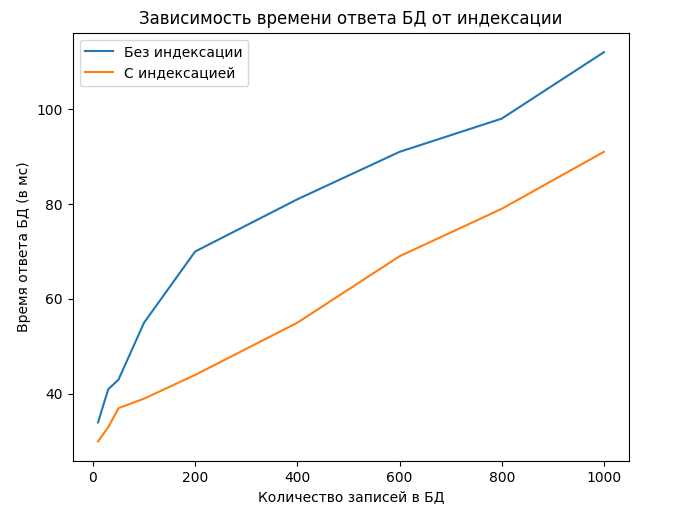
\includegraphics[height=10cm, width=\linewidth]{inc/graph.png}
	\end{center}
	\caption{График зависимости времени ответа БД от индексации}
\end{figure}
\FloatBarrier

Как видно, индексация позволила уменьшить время ответа. При $N=600$ время сократилось на $30\%$, при $N=800$ -- на $20\%$. При этом индексированная таблица возвращала результат быстрее при всех измерениях.